\documentclass[12pt]{article}
\usepackage[english]{babel}
\usepackage{graphicx, amsmath, amsfonts, amsthm, mathtools, listings, color, caption, rotating, subfigure, fullpage, textcomp, enumerate, float, listings, MnSymbol, wasysym}

\lstset{
	language=R,
	keywordstyle=\bfseries\ttfamily\color[rgb]{0,0,1},
	identifierstyle=\ttfamily,
	commentstyle=\color[rgb]{0.133,0.545,0.133},
	stringstyle=\ttfamily\color[rgb]{0.627,0.126,0.941},
	showstringspaces=false,
	basicstyle=\tiny,
	numberstyle=\scriptsize,
	numbers=left,
	stepnumber=1,
	numbersep=10pt,
	tabsize=2,
	breaklines=true,
	breakatwhitespace=false,
	aboveskip={1.5\baselineskip},
  columns=fixed,
  upquote=true,
  extendedchars=true,
}

\begin{document}
\begin{center}
STA250, Homework 1 \\
Christopher Aden\\
October 21, 2013\
\end{center}

\section*{Proof that Gibbs Sampler Will Converge:}
\subsection*{Part B}
Let $p(\underline{x})$ denote the probability density function of a vector of random variables $x_1, \dots, x_p$. We will assume that the Markov Chain that results from running the Gibbs Sampler is ergodic. We want to show that the stationary distribution of the $p$-component Gibbs sampler is indeed this target distribution $p(\underline{x})$.

To avoid having to write a bunch of stuff in $\LaTeX$, let me introduce a couple pieces of notational shorthand. Let $x^t$ denote the $t$-th iteration of the Gibbs Sampler (\textbf{not} $x$ to the power $t$!). Additionally, $x_{[i:j]} = (x_i, x_{i+1}, \dots, x_{j-1}, x_j)$, just like the slice operation in Python or the colon function in R.

By the assumption of ergodicity, we know that the Markov Chain formed by the Gibbs Sampler, $\underline{x}^1, \underline{x}^2, \dots,$ converges to a stationary distribution, denoted by $\pi(\underline{x})$ in the notes. In the continuous state space case, it is a property of a stationary Markov Chain that 
\[ \pi (\underline{y}) = \int_{\mathbb{R}^p} \pi (\underline{x}) p(\underline{x}, \underline{y}) d \underline{x}.\] 
That is, we must have that the probability of arriving at state $\underline{y}$ is the integral of the probability of being at state $\underline{x}$ times the probability of moving from state $\underline{x}$ to state $\underline{y}$.

This will require only two steps: deriving a closed form for the transition density $p(\underline{x}, \underline{y})$ and showing that the (multivariate) integral of the stationary distribution times the transition density gives us the stationary distribution. We will assert that one such stationary distribution that satisfies this property is the target distribution, then use the uniqueness of the stationary distribution to claim the target distribution is the unique stationary distribution.

\textbf{Transition Density:} What is the density of $\underline{x}^{t+1}$, given $\underline{x^t}$? For this, by conditional expectation,
\begin{align*}
p(\underline{x}^{t+1} | \underline{x}^{t}) &= p(x_1^{t+1}, x_2^{t+1}, \dots, x_p^{t+1} | \underline{x}^{t}) \\
&= p(x_1^{t+1} | \underline{x}^{t}) \cdot p(x_2^{t+1}, \dots, x_p^{t+1} | x_1^{t+1}, \underline{x}_{[2:p]}^{t}) \\
&= p(x_1^{t+1} | \underline{x}^{t}) \cdot p(x_2^{t+1} | x_1^{t+1}, \underline{x}_{[2:p]}^{t}) \cdot p(x_3^{t+1}, \dots, x_p^{t+1} | x_{[1:2]}^{t+1}, \underline{x}_{[3:p]}^{t}) \\
&= \dots \textrm{(Repeated conditioning, unrolling each term conditioned on all the rest,)} \\
&= p(x_1^{t+1} | \underline{x}^t) \cdot p(x_2^{t+1} | x_1^{t+1}, \underline{x}_{[2:p]}^{t}) \dots p(x_p^{t+1} | \underline{x}_{[1:p-1]}^{t+1}, x_p^t)
\end{align*}
Intuitively, you can think of this as similar to what the Gibbs Sampler does. The distribution of the joint is the product of the conditionals of each random variable at the current iteration, given the variables already drawn in the current iteration and the previous iteration for the variables not yet drawn in the current iteration.

\textbf{Stationarity:} The target distribution $p(\underline{x})$ is stationary iff
\begin{align*}
p(\underline{x}^{t+1}) &= \int_{\mathbb{R}^p} p(\underline{x}^{t}) p(\underline{x}^{t+1}| \underline{x}^{t}) d \underline{x}^t, \forall \underline{x}^t \in \mathbb{R}^p. \\
&= \int_{\mathbb{R}} \cdots \int_{\mathbb{R}} p(x_1^{t}, x_2^{t}, \dots, x_p^{t}) p(x_1^{t+1}, x_2^{t+1}, \dots, x_p^{t+1} | x_1^{t}, x_2^{t}, \dots, x_p^{t}) dx_1^t dx_2^t \cdots dx_p^t,
\end{align*}
for all $x_i^t \in \mathbb{R}$, $i=1, \dots, p$. Recall that $f(y) = \int_\mathbb{R} f(x,y) dx = \int_\mathbb{R} f(x) \cdot f(y|x) dx$ for arbitrary real-valued random variables $y$ and $x$. The above integral can be seen to be the product of a marginal of $\underline{x}^t$ and the conditional of $\underline{x}^{t+1}$ given $\underline{x}^t$, integrated over the entire parameter space of $\underline{x}^t$. By similar logic to my univariate example earlier in the paragraph, we see that the result of this will be the marginal distribution of $\underline{x}^{t+1}$.
\[ \Rightarrow \int_{\mathbb{R}^p} p(\underline{x}^{t}) p(\underline{x}^{t+1}| \underline{x}^{t}) d \underline{x}^t = p(\underline{x}^{t+1}). \]
Combining the uniqueness of the stationary distribution with the stationarity of the target distribution, we have that the Gibbs Sampler Markov Chain converges to the target distribution. $\blacksquare$
\subsection*{Part A}
First, a story: An engineer and a mathematician shared an apartment. Their kitchen was equipped with an electric stove, and every morning someone had placed a pot of water on the back-right burner so they could make coffee. They both knew what knob turned on this burner. One morning the engineer came into the kitchen and found the pot was on the front-left burner. He got out the stove's schematics and followed the wiring diagram and finally figured out which knob turned on this burner and he then used that knob and made the coffee. The next morning the mathematician came in and also found the pot on the front-left burner. He moved the pot to the back-right burner, thereby reducing the problem to one which he had already solved.

\noindent \textbf{Proof:} Let $p=2$. Refer to Part B. $\blacksquare$

\section*{Metropolis-Hastings with Simulated 2-dimensional Parameter}
Being unable to directly sample the posterior distribution acquired by a multivariate normal prior and a binomial likelihood, we are reduced to more computational methods. Assume our likelihood and prior are
\begin{align*}
& \beta \sim N(\mu_0, \Sigma_0) \\
& y_{i} | \beta \sim \textrm{Bin}(m_{i},\textrm{expit}(x_{i}^{T}\beta)) , \qquad i=1, \ldots, n,
\end{align*}
where $\text{expit}(u) = \exp(u) / (1+\exp(u))$. For tractability, assume the responses are conditionally independent given $\beta$.

The posterior is thus
	\begin{align*}
	f(\underline{\beta} | \underline{y}) &\propto f(\underline{\beta}) \cdot \prod_{i=1}^n f(y_i | \beta) \quad \text{(by the cond. indep. of } y_i\text{ and Bayes' Theorem)} \\
	&= N(\mu_0, \Sigma_0) \cdot \prod_{i=1}^n \textrm{Bin}(m_{i},\textrm{ expit}(x_{i}^{T}\beta)) \\
	&\propto \exp{ \left( -\frac{1}{2} (\beta-\mu_0)^T \Sigma_0^{-1} (\beta-\mu_0) \right) } \prod_{i=1}^n \binom{m_i}{y_i} \text{expit}(x_i^T \beta)^{y_i} (1-\text{expit}(x_i^T \beta))^{m_i - y_i} \\
	&\propto \exp \left( -\frac{1}{2} (\beta-\mu_0)^T \Sigma_0^{-1} (\beta-\mu_0) \right) \prod_{i=1}^n \frac{\exp(x_i^T \beta)^{y_i}}{1+\exp(x_i^T \beta)^{y_i}} \frac{1}{1 + \exp(x_i^T \beta)^{m_i - y_i}} \\
	&= \exp \left( -\frac{1}{2} (\beta-\mu_0)^T \Sigma_0^{-1} (\beta-\mu_0) \right) \prod_{i=1}^n \frac{\exp(x_i^T \beta)^{y_i}}{1+\exp(x_i^T \beta)^{y_i}} \frac{1 + \exp(x_i^T \beta)^{y_i}}{1 + \exp(x_i^T \beta)^{m_i}} \\
	&= \exp \left( -\frac{1}{2} (\beta-\mu_0)^T \Sigma_0^{-1} (\beta-\mu_0) \right) \prod_{i=1}^n \frac{\exp(x_i^T \beta)^{y_i}}{1+\exp(x_i^T \beta)^{m_i}} \\
	\end{align*}
This can be simplified further, but there's not much point. This distribution has no closed form in $\beta$. We cannot directly sample from it, so we must apply Metropolis-Hastings.
	\begin{enumerate}
	\item Specify a starting point for the Markov Chain, $\beta^0$.
	\item At each increment $i$ in the Markov Chain, propose a new value, $\beta^*$, centered on the previous one, $\beta^i$.
	\item Compute the probability of the posterior at the candidate value $p(\beta^* | \underline{y})$ (derived up to proportionality above), as well as the posterior at the current value $p(\beta^i | \underline{y})$. In R, we work up to proportionality, so this is as simple as multiplying the prior by the likelihood, \texttt{dmvnorm} by \texttt{dbinom}. For stability reasons, we work on the log scale, so we'll add the log-prior and the log-likelihood to get the log-posterior.
	\item Compute $\alpha^* = \frac{p(\beta^* | \underline{y})}{p(\beta^i | \underline{y})}$.
	\item Draw $U \sim U(0,1)$. If $U \leq \alpha^*$, set $\beta^{i+1} = \beta^*$. Else, $\beta^{i+1} = \beta^{i}$. Again, because of the log-scale, we can compare a log-uniform against the difference of the log-posterior at the candidate to the log-posterior at the current value of the Markov Chain, and the results will be equivalent with a greatly-reduced concern for numerical inaccuracy.
	\item The vector $\beta^i, i=1, \dots, n$ represents dependent draws from the target distribution $p(\beta | \underline{y})$. 
	\end{enumerate}
This algorithm has a ton of knobs and switches to play with. The following summarizes some of the parameters I use to make the algorithm more efficient.
\begin{description}
\item[Starting Values:] $\beta^0 = \hat{\beta}$, the MLE of the data, was chosen. We can think of this as being close to the posterior mode if we had an uninformative prior distribution. It can be shown that as the sample size increases, the effect of the prior diminishes for any non-degenerate prior, so for our sample size, the MLE will be quite close to the posterior mode. Using the MLE is a sensible choice if the sample size is large enough that the likelihood carries more weight in the posterior than the prior does.

\item[Proposal Distribution] The proposal is generated from the proposal distribution, which I chose to be a bivariate normal, centered on the previous value, with a covariance matrix $v^2 \Sigma$, where $v^2$ is a tuning parameter that changes to give a suitable acceptance rate for samples. $\Sigma$ is the estimated covariance matrix using a Frequentist logistic regression, which, for large enough sample size, closely models the structure of the posterior covariance. The reason for choosing a bivariate normal as my proposal distribution was out of simplicity. Using the bivariate normal, the probably of going from the candidate value to the current value is the same as going from current to candidate, a property called symmetry. This simplifies the calculation of the Metropolis-Hastings acceptance statistic. The choice of that strange form for the covariance matrix is an attempt at mimicking the variance of the posterior distribution. I acquired this matrix by fitting a logistic regression in R with \texttt{glm}, then using its estimate for the covariance as my proxy for the posterior variance.

\item[Tuning Process] Every so often, we will go through a retuning process. It is possible that the proposal distribution does not have an appropriate variance. Too high a variance and we will propose bad values, rejecting too often and ending up with lots of redundant draws. If the variance is too small, we will stay in relatively the same spot, not exploring the space effectively, accepting too often. In both cases, we end up with a very small effective sample size, and gaining very little additional information on each draw. The solution to this problem is to keep track of our acceptance rates and make sure it stays within a good acceptance rate window. I chose 20\% to 50\% for this 2-dimensional example. This comes based on heuristic moreso than any analytical reason. This ended up being pretty reasonable, so I stuck with it. If the acceptance rate fell outside this band, I adjusted the proposal variance by a scalar factor of $v_i^{2} = \exp{(3 \cdot (\text{acceptance}-\text{ideal}))}$, where $v_i^2$ is the scalar proposed during this tuning period (the previous tuning period times the scaling factor). Acceptance is the acceptance ratio, and ideal is the ideal accept rate. For the two-dimensional case, I chose 30\%, which is a reasonable balance between accepting and rejecting. If the acceptance rate is higher than 30\%, this scaling will increase the proposal variance (to make more adventurous jumps). If the acceptance is less, the scaling will decrease the variance. The coefficient of 3 was chosen as a factor of how much to scale by each time and was chosen by hand-tuning heuristically. 

\item[Number of Iterations] Computing power is inexpensive in 2013. As long as I have other things to do, I would rather have the computer spend two hours running my code than have to spend 30 minutes of my time optimizing the program to make it run quicker. Consistent with that philosophy, I spend very little time choosing a decent number of iterations. A couple million samples takes less than 10 minutes on my Linux machine, with a retuning every thousand observations up to the burn-in.

\item[Burn-In Period] Like the number of iterations, the burn-in is somewhat of a non-issue. I cleverly chose to start at the MLE of the likelihood, which means my Markov Chain was pointed at the correct position from the very beginning. I could've chosen a very small burn-in if I wanted, but I also needed to adjust the proposal variance, so I set the burn-in to be around $10,000$. If I could've adjusted the variance on-the-fly \emph{and} kept those draws instead of burning them, I could've made the burn-in period far less. I hit stationarity after less than a thousand draws most times.
\end{description}

For this simple 2-dimensional problem, Metropolis-Hastings makes short work of sampling the posterior. While the effective sample size is only about 17\% of the total sample size, this is good enough if we run enough iterations of the algorithm. We can thin the data (taking only every $k^{th}$ iteration) if we are worried about autocorrelation between samples, but I didn't bother for only two dimensions. Looking at the traceplots, we see that stationarity has been attained. 
\begin{figure}[H] \center
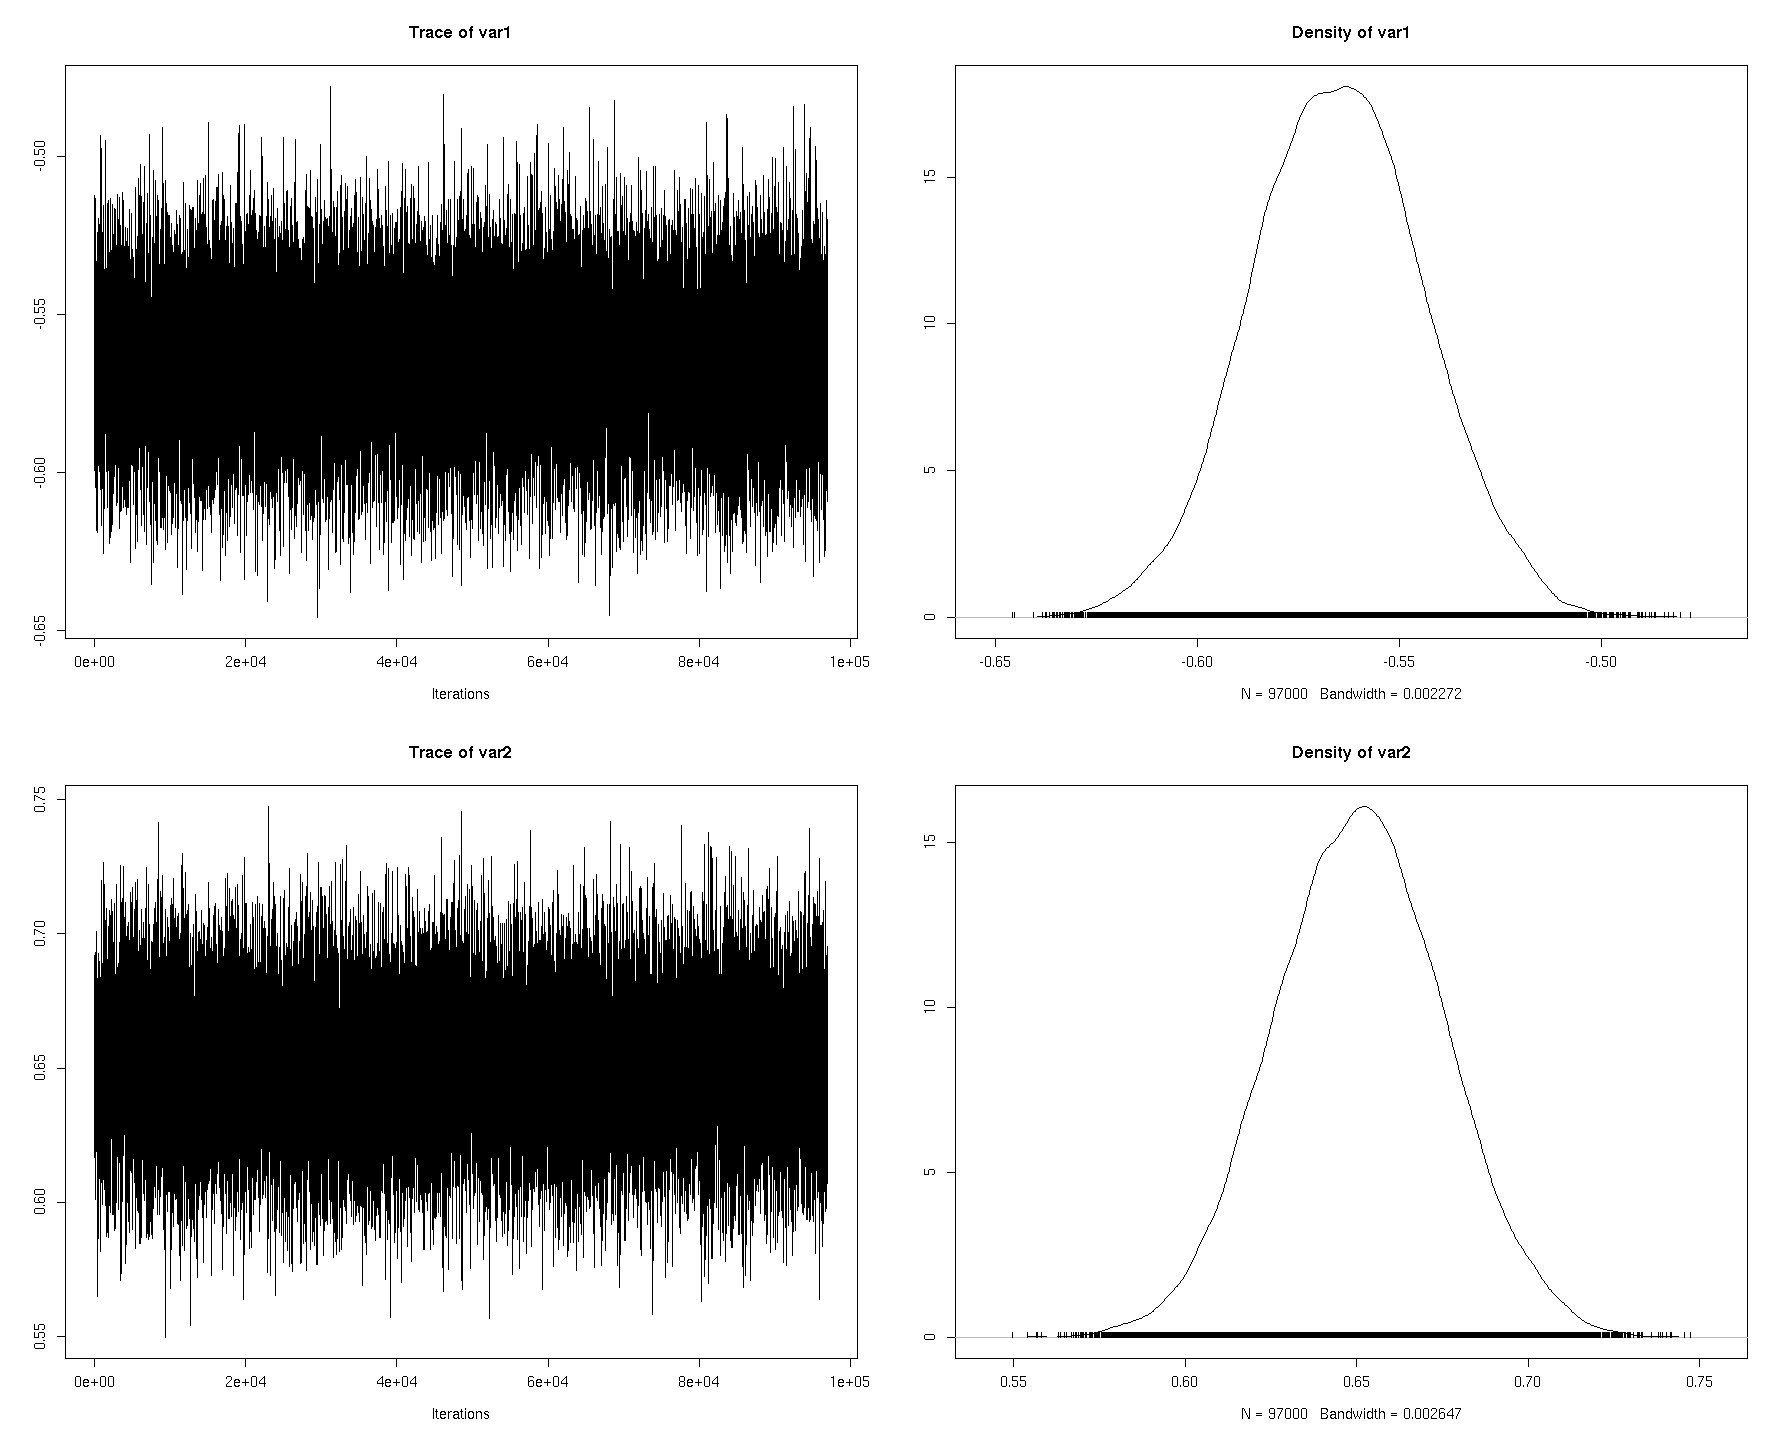
\includegraphics[scale=.20]{MCMC_p2.jpeg}
\caption*{Trace and density plots for $(\beta_1, \beta_2)$, $n=10^5$, $\text{burn}=3000$, $\text{retune}=100$.}
\end{figure}
A similar picture can be seen on the other 200 datasets generated on the compute cluster. On the topic of coverage probabilities, you may take a look at the coverage summaries. Things turned out okay. Keep in mind that there is randomness associated with the Markov Chain. Running the simulation another time changes the coverage probabilities.

\begin{figure}[H] \center
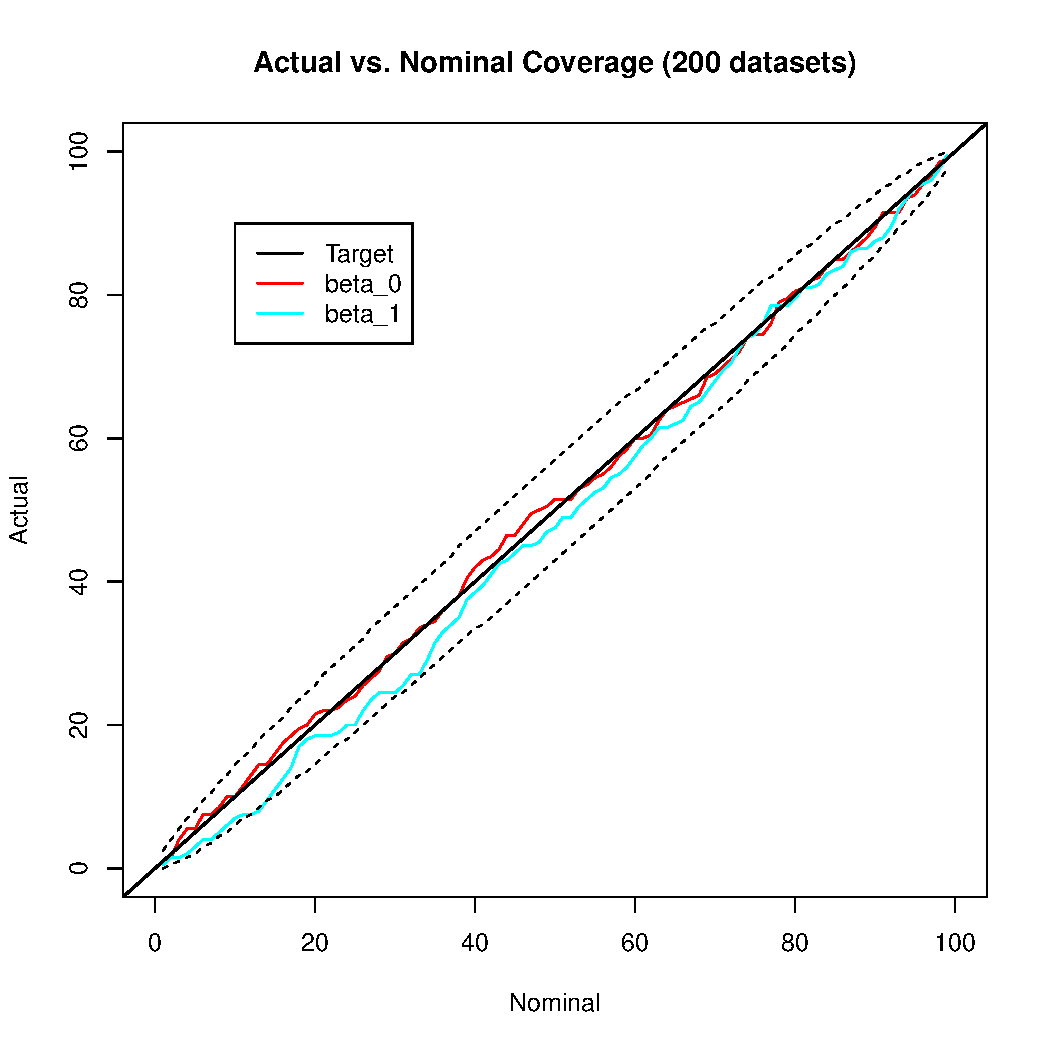
\includegraphics[scale=.65]{coverage_line_plot.pdf}
\caption*{Coverage Line Plot for $(\beta_1, \beta_2)$, $n=5 \cdot 10^5$, $\text{burn}=10^4$, $\text{retune}=10^3$.}
\end{figure}

\begin{table}[H] \center
\begin{tabular}{rrr} \hline
& $\beta_0$ & $\beta_1$ \\ \hline
p\_01 & 0.01 & 0.01 \\ 
p\_05 & 0.06 & 0.03 \\ 
p\_10 & 0.10 & 0.07 \\ 
p\_25 & 0.24 & 0.20 \\ 
p\_50 & 0.52 & 0.47 \\ 
p\_75 & 0.74 & 0.74 \\ 
p\_90 & 0.90 & 0.88 \\ 
p\_95 & 0.94 & 0.95 \\ 
p\_99 & 0.99 & 0.99 \\ \hline
\end{tabular}
\caption*{Coverage Probabilities for $(\beta_0, \beta_1)$.}
\end{table}

\section*{Metropolis-Hastings with 11-dimensional Parameter on Real Data}
The previous approach did not work very well on this particular problem (wait for the punchline after the table). I tried do it in the same fashion, with 100,000 iterations, a burn-in of 20,000, an acceptance range between 10\% and 30\% to accommodate the more frequent number of rejections, the algorithm finished quickly, but the effective sample size for the Texture variable was not much larger than 5. In the interest of not re-writing my Metropolis-Hastings code from Problem 2, I ramped up the iterations to 5,000,000 (\emph{five million!}). The effective sample size of the Texture variable (X11) was still only 10.

The dimension of the parameter space is partially to blame. It's difficult to propose plausible values in 11-dimensional space and have them be more likely than another previously-selected value. But the ``Curse of Dimensionality'' cannot fully explain the difficulty of sampling the $\beta$s in this problem. Looking at the covariance matrix of the 11 parameters, we can see where we might have trouble.
\begin{table}[H] \center 
\begin{tabular}{|cccccccccccc|} \hline
& $\beta_1$ & $\beta_2$ & $\beta_3$ & $\beta_4$ & $\beta_5$ & $\beta_6$ & $\beta_7$ & $\beta_8$ & $\beta_9$ & $\beta_{10}$ & $\beta_{11}$ \\ \hline
& 165.19 & 0.0003 & 413.82 & 813.91 & 65.94 & 7319.94 & 0.26 & 13.81 & 1021.12 & 113.01 & 0.004 \\ \hline
\end{tabular}
\caption*{Variances for MLEs $\hat{\beta_i}$, $i=1, \dots, 11$.}
\end{table}
The scale is simply ridiculous! Variables X2 (area), X7 (perimeter), and X11 (texture) are on the order of tenths to thousandths, while X6 (fracdim) and X9 (smoothness) are in the thousands. Between the smallest-varied and largest-varied variables, we're looking at a six order of magnitude difference! This makes it very hard to tune our proposal distribution. However, a clever choice of proposal distribution solves a number of problems. I was initially unable to get the MH algorithm to converge correctly with this complicated space. Using the estimated covariance matrix created from a logistic regression solved a large part of the problem, but was still not enough until about 10pm sitting in my office, I realized I had been using the wrong prior ($\frac{1}{1000} \cdot I_{11} \neq 1000 \cdot I_{11}$)! Changing the code drastically increased my effective sample size to the point that Metropolis-Hastings became a viable option for sampling an 11-dimensional parameter space. The convergence was not as nice as the 2-dimensional case, but people who don't want to spend extra time re-factoring optimized code can't be choosers. Running the chain a long time handily solves this problem anyway.
Let's talk about the autocorrelation. Using built-in R function \texttt{acf()}, computing the lag-1 autocorrelation is trivial.
\begin{table}[H] \center
\begin{tabular}{|ccccccccccc|} \hline
$\beta_1$ & $\beta_2$ & $\beta_3$ & $\beta_4$ & $\beta_5$ & $\beta_6$ & $\beta_7$ & $\beta_8$ & $\beta_9$ & $\beta_{10}$ & $\beta_{11}$ \\ \hline
0.95 & 0.96 & 0.94 & 0.93 & 0.96 & 0.83 & 0.96 & 0.96 & 0.93 & 0.96 & 0.96 \\ \hline
\end{tabular}
\caption*{The Lag-1 autocorrelation for each $\beta_i$.}
\end{table}
Terrible. Each draw is very correlated to the previous draw. One simple and slightly naive way to handle this problem is to thin the samples, removing every $k^{th}$ observation. Thinning will reduce the effective sample size, but since I ran the chain for half a million iterations, I can afford to lose 98\% of my Markov Chain iterations to cut down the autocorrelation.
\begin{table}[H] \center
\begin{tabular}{|ccccccccccc|} \hline
$\beta_1$ & $\beta_2$ & $\beta_3$ & $\beta_4$ & $\beta_5$ & $\beta_6$ & $\beta_7$ & $\beta_8$ & $\beta_9$ & $\beta_{10}$ & $\beta_{11}$ \\ \hline
0.16 & 0.19 & 0.12 & 0.05 & 0.14 & 0.05 & 0.20 & 0.18 & 0.01 & 0.20 & 0.14 \\ \hline
\end{tabular}
\caption*{The Lag-1 autocorrelation for each $\beta_i$ using 50-thinning.}
\end{table}

\begin{table}[H] \center
\begin{tabular}{|ccccccccccc|} \hline
$\beta_1$ & $\beta_2$ & $\beta_3$ & $\beta_4$ & $\beta_5$ & $\beta_6$ & $\beta_7$ & $\beta_8$ & $\beta_9$ & $\beta_{10}$ & $\beta_{11}$ \\ \hline
0.08 & 0.05 & -0.04 & -0.02 & 0.08 & -0.05 & 0.02 & 0.02 & -0.01 & 0.08 & -0.01 \\ \hline
\end{tabular}
\caption*{The Lag-1 autocorrelation for each $\beta_i$ using 100-thinning.}
\end{table}
The 100-thinned version is basically uncorrelated at this point. The effective sample size demonstrated this, as most variables had effective sample sizes that were very close to actual number of thinned samples. For my large iteration choice, this yielded 5,000 uncorrelated samples from the posterior, which was good enough for me. In hindsight, I could've been fine running 50,000 iterations and still had 500 uncorrelated samples.

Convince yourself from my traceplots that the chain has good convergence. 
\begin{figure}[H] \center
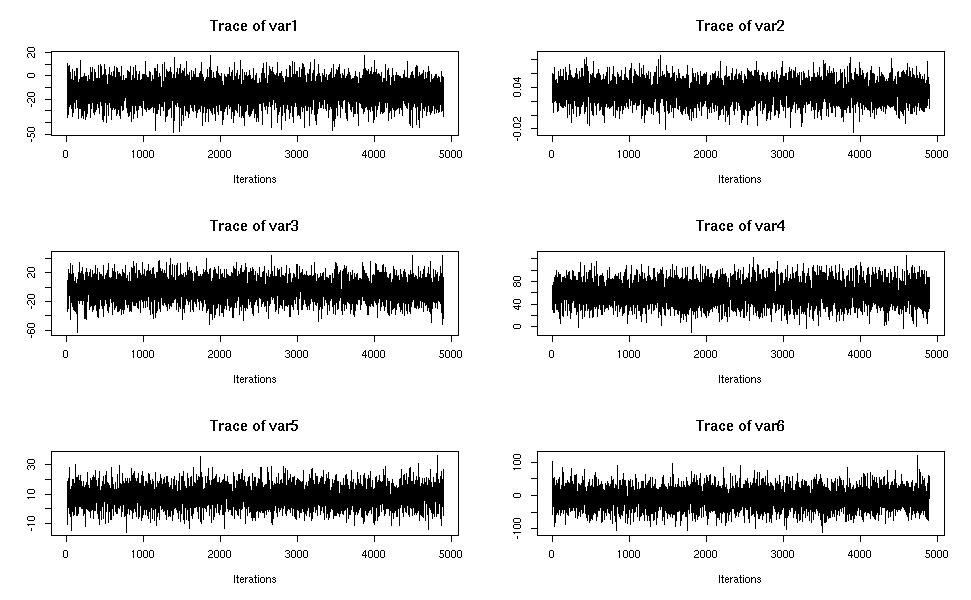
\includegraphics[scale=.45]{MCMC_p3_1.jpeg}
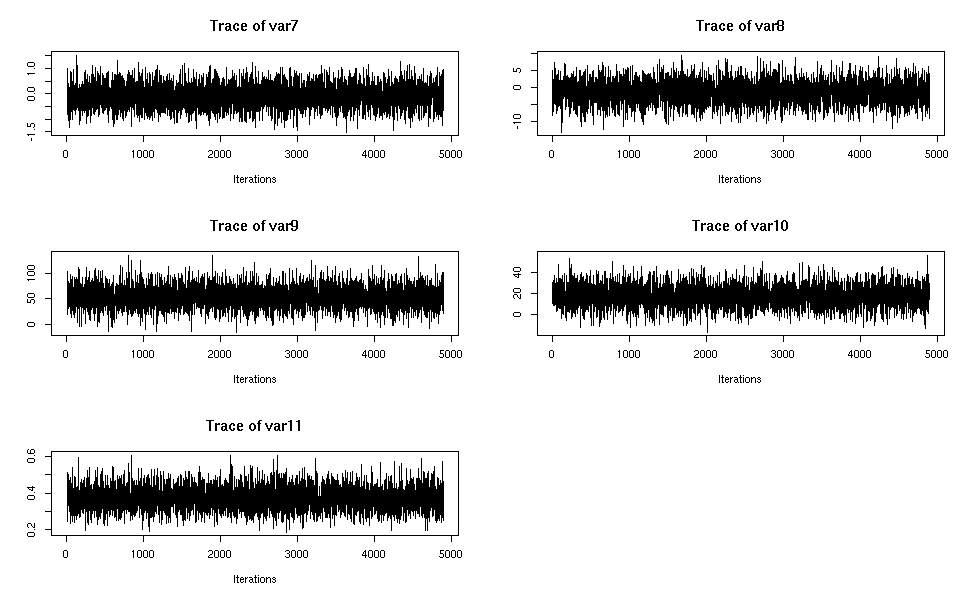
\includegraphics[scale=.45]{MCMC_p3_2.jpeg}
\caption*{Trace and density plots for $(\beta_1, \dots, \beta_{11})$, $n=5\cdot 10^5$, $\text{burn}=10^4$, $\text{retune}=100$.}
\end{figure}

Next, we consider the problem of variable selection. Bayesian variable selection works in a different way from Frequentist variable selection, since we don't have the same kind of Neyman-Pearson formulation that we did before--the concept of controlling a Type 1 error for a model isn't as meaningful. One approach is simply to look at the posterior credible intervals and see which ones contain zero, because while the magnitude of each posterior parameter does depend on the scaling of each variable, whether the posterior intervals contain zero is only very weakly dependent on the scaling. From the table, it seems the most important variables (the ones that don't contain zero)  are $\beta_4$, $\beta_9$, and $\beta_{11}$ (concave points, smoothness, and texture, respectively).  
\begin{table}[H] \center
\begin{tabular}{|c|ccccccccccc|} \hline
 & $\beta_1$ & $\beta_2$ & $\beta_3$ & $\beta_4$ & $\beta_5$ & $\beta_6$ & $\beta_7$ & $\beta_8$ & $\beta_9$ & $\beta_{10}$ & $\beta_{11}$ \\  \hline
2.5\% & -36.31 & 0.00 & -30.85 & 19.69 & -6.33 & -67.32 & -0.85 & -8.15 & 15.52 & -0.66 & 0.26 \\ 
  97.5\% & 4.10 & 0.06 & 22.50 & 98.34 & 23.22 & 51.30 & 0.84 & 4.49 & 87.96 & 36.64 & 0.49 \\ \hline
\end{tabular}
\caption*{95\% Central Credible Interval} 
\end{table}
 
Finally, I will talk about checking our model. Model checking in Bayesian inference is done through posterior predictive checking. This procedure involves drawing parameters $\underline{\beta}$ from the posterior distribution, then generating simulated data from the assumed likelihood, given those posterior values as the parameters. If the model is an accurate representation of the data, the posterior predictive distributions should not be all that different from the true data, which we can corroborate using summary statistics (mean, median, variance, and the like). Our algorithm is as follows:
\begin{enumerate}
\item Draw $\underline{\beta}^i$ from the posterior, $p(\underline{\beta} | \underline{y})$, for $i=1, \dots, M$. 
\item Simulate $M$ datasets $\tilde{y}^i$, where $\tilde{y}^i \sim \text{Bin}(m_i, \text{expit}(X^T \beta^i))$.
\item Compute a summary statistic on each dataset, $T(\tilde{y}^i)$, then create a histogram with the $M$ summary statistics.
\end{enumerate}

If the model is correct, the true summary statistic should sit somewhere near the center of the histogram (or at least not in the far tails of the histogram). Since the likelihood is Bernoulli data, minimum and maximum statistics are not useful. I went with the mean and the variance, and we can see from the plots that the binomial likelihood model is quite sensible in this case.
\begin{figure}[H] \center
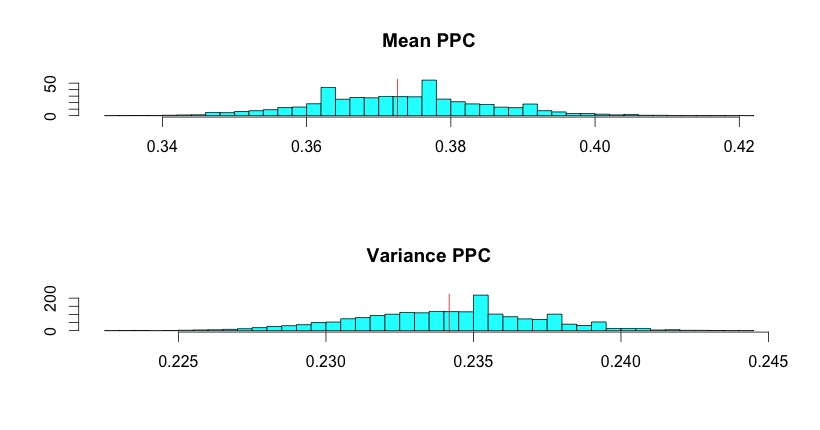
\includegraphics[scale=.50]{MCMC_p3_3.jpeg}
\caption*{Posterior Predictive Checks for the Mean and Variance}
\end{figure}

The red line indicates the true mean and variance. The mean was chosen as a measure of center, and the variance was the choice for measuring dispersion. There is an inflexible relationship between the mean and the variance with the binomial, so if another model was more appropriate, checking both variance and mean could have given some insight. As it turns out, the lines sit very closely to the middle of both histograms, leading us to believe that the model is quite sound as a way of modeling both the mean and the variance. It is possible that the model is not a good fit through some other summary statistic. A more thorough method would be to look at a number of quantiles as the summary statistics. This provides a very accurate picture of both the tails and the center of the model. Similar to the QQ Plot, the posterior predictive quantiles ought to match up against the true corresponding quantiles if the model is valid (think of this as as many histograms as there are quantiles). In the interest of parsimony, I chose only a measure of center and a measure of dispersion.

\section*{R Source Code}
Helper\_functions is a script containing the majority of the algorithms I used to do Bayesian Logistic regression. It contains basic functions, as well as my Metropolis Hastings implementation, computation of quantiles, and posterior predictive checks.
\lstinputlisting{"helper_functions.R"}

The BLR\_Fit file contains the code to run the simulations when the true value was known. It outputs a matrix containing the quantiles for each of the two parameters.
\lstinputlisting{"BLR_fit.R"}

The Cancer file handles the import and cleaning of the cancer data, along with the creation of graphs and the MCMC for the data set. At the end, it produces effective sample size, convergence plots, and does a little bit of model checking using posterior predictive checks.
\lstinputlisting{"Cancer.R"}
\end{document} 